%package list
\documentclass{article}
\usepackage[top=3cm, bottom=3cm, outer=3cm, inner=3cm]{geometry}
\usepackage{multicol}
\usepackage{graphicx}
\usepackage{url}
%\usepackage{cite}
\usepackage{hyperref}
\usepackage{array}
%\usepackage{multicol}
\newcolumntype{x}[1]{>{\centering\arraybackslash\hspace{0pt}}p{#1}}
\usepackage{natbib}
\usepackage{pdfpages}
\usepackage{multirow}
\usepackage[normalem]{ulem}
\useunder{\uline}{\ul}{}
\usepackage{svg}
\usepackage{xcolor}
\usepackage{listings}
\lstdefinestyle{ascii-tree}{
    literate={├}{|}1 {─}{--}1 {└}{+}1 
  }
\lstset{basicstyle=\ttfamily,
  showstringspaces=false,
  commentstyle=\color{red},
  keywordstyle=\color{blue}
}
%\usepackage{booktabs}
\usepackage{caption}
\usepackage{subcaption}
\usepackage{float}
\usepackage{array}

\newcolumntype{M}[1]{>{\centering\arraybackslash}m{#1}}
\newcolumntype{N}{@{}m{0pt}@{}}


%%%%%%%%%%%%%%%%%%%%%%%%%%%%%%%%%%%%%%%%%%%%%%%%%%%%%%%%%%%%%%%%%%%%%%%%%%%%
%%%%%%%%%%%%%%%%%%%%%%%%%%%%%%%%%%%%%%%%%%%%%%%%%%%%%%%%%%%%%%%%%%%%%%%%%%%%
\newcommand{\itemEmail}{rcompanocca@unsa.edu.pe}
\newcommand{\itemStudent}{Roni Companocca Checco}
\newcommand{\itemCourse}{Programación}
\newcommand{\itemCourseCode}{20210558}
\newcommand{\itemSemester}{II}
\newcommand{\itemUniversity}{Universidad Nacional de San Agustín de Arequipa}
\newcommand{\itemFaculty}{Facultad de Ingeniería de Producción y Servicios}
\newcommand{\itemDepartment}{Departamento Académico de Ingeniería de Sistemas e Informática}
\newcommand{\itemSchool}{Escuela Profesional de Ingeniería de Sistemas}
\newcommand{\itemAcademic}{2023 - B}
\newcommand{\itemInput}{Del 13 Noviembre 2023}
\newcommand{\itemOutput}{Al 18 Noviembre 2023}
\newcommand{\itemPracticeNumber}{15}
\newcommand{\itemTheme}{Mecanismos de Agregación, Composición, Herencia (II)}
%%%%%%%%%%%%%%%%%%%%%%%%%%%%%%%%%%%%%%%%%%%%%%%%%%%%%%%%%%%%%%%%%%%%%%%%%%%%
%%%%%%%%%%%%%%%%%%%%%%%%%%%%%%%%%%%%%%%%%%%%%%%%%%%%%%%%%%%%%%%%%%%%%%%%%%%%

\usepackage[english,spanish]{babel}
\usepackage[utf8]{inputenc}
\AtBeginDocument{\selectlanguage{spanish}}
\renewcommand{\figurename}{Figura}
\renewcommand{\refname}{Referencias}
\renewcommand{\tablename}{Tabla} %esto no funciona cuando se usa babel
\AtBeginDocument{%
	\renewcommand\tablename{Tabla}
}

\usepackage{fancyhdr}
\pagestyle{fancy}
\fancyhf{}
\setlength{\headheight}{30pt}
\renewcommand{\headrulewidth}{1pt}
\renewcommand{\footrulewidth}{1pt}
\fancyhead[L]{\raisebox{-0.2\height}{
\includegraphics[width=3cm]{logo_episunsa.png}}}
\fancyhead[C]{\fontsize{7}{7}\selectfont	\itemUniversity \\ \itemFaculty \\ \itemDepartment \\ \itemSchool \\ \textbf{\itemCourse}}
\fancyhead[R]{\raisebox{-0.2\height}{
\includegraphics[width=1.2cm]{abet.png}}}
\fancyfoot[L]{Estudiante Roni Companocca Checco}
\fancyfoot[C]{\itemCourse}
\fancyfoot[R]{Página \thepage}

% para el codigo fuente
\usepackage{listings}
\usepackage{color, colortbl}
\definecolor{dkgreen}{rgb}{0,0.6,0}
\definecolor{gray}{rgb}{0.5,0.5,0.5}
\definecolor{mauve}{rgb}{0.58,0,0.82}
\definecolor{codebackground}{rgb}{0.95, 0.95, 0.92}
\definecolor{tablebackground}{rgb}{0.8, 0, 0}

\lstset{frame=tb,
	language=bash,
	aboveskip=3mm,
	belowskip=3mm,
	showstringspaces=false,
	columns=flexible,
	basicstyle={\small\ttfamily},
	numbers=none,
	numberstyle=\tiny\color{gray},
	keywordstyle=\color{blue},
	commentstyle=\color{dkgreen},
	stringstyle=\color{mauve},
	breaklines=true,
	breakatwhitespace=true,
	tabsize=3,
	backgroundcolor= \color{codebackground},
}

\begin{document}
	
	\vspace*{10px}
	
	\begin{center}	
		\fontsize{17}{17} \textbf{ Informe de Laboratorio \itemPracticeNumber}
	\end{center}
	\centerline{\textbf{\Large Tema: \itemTheme}}
	%\vspace*{0.5cm}	

	\begin{flushright}
		\begin{tabular}{|M{2.5cm}|N|}
			\hline 
			\rowcolor{tablebackground}
			\color{white} \textbf{Nota}  \\
			\hline 
			     \\[30pt]
			\hline 			
		\end{tabular}
	\end{flushright}	

	\begin{table}[H]
		\begin{tabular}{|x{4.7cm}|x{4.8cm}|x{4.8cm}|}
			\hline 
			\rowcolor{tablebackground}
			\color{white} \textbf{Estudiante} & \color{white}\textbf{Escuela}  & \color{white}\textbf{Asignatura}   \\
			\hline 
			{\itemStudent \par \itemEmail} & \itemSchool & {\itemCourse \par Semestre: \itemSemester \par Código: \itemCourseCode}     \\
			\hline 			
		\end{tabular}
	\end{table}		
	
	\begin{table}[H]
		\begin{tabular}{|x{4.7cm}|x{4.8cm}|x{4.8cm}|}
			\hline 
			\rowcolor{tablebackground}
			\color{white}\textbf{Laboratorio} & \color{white}\textbf{Tema}  & \color{white}\textbf{Duración}   \\
			\hline 
			\itemPracticeNumber & \itemTheme & 04 horas   \\
			\hline 
		\end{tabular}
	\end{table}
	
	\begin{table}[H]
		\begin{tabular}{|x{4.7cm}|x{4.8cm}|x{4.8cm}|}
			\hline 
			\rowcolor{tablebackground}
			\color{white}\textbf{Semestre académico} & \color{white}\textbf{Fecha de inicio}  & \color{white}\textbf{Fecha de entrega}   \\
			\hline 
			\itemAcademic & \itemInput &  \itemOutput  \\
			\hline 
		\end{tabular}
	\end{table}

    \section{TAREA}
	\begin{itemize}	
    \subsection{Objetivos:}
		\item Que el alumno demuestre poder crear “clases definidas por el programador”
		\item Implementar métodos para las clases definidas por el programador
        \item Utilizando atributos que son otros objetos. Agregación, composición, herencia.
       
    \subsection{Competencias a alcanzar:}
		\item Diseña, responsablemente, sistemas, componentes o procesos para satisfacer necesidades dentro de restricciones realistas: económicas, medio ambientales, sociales, políticas, éticas, de salud, de seguridad, manufacturación y sostenibilidad. 
        \item Aplica de forma flexible, técnicas, métodos, principios, normas, estándares y herramientas de ingeniería necesarias para la construcción de software e implementación de sistemas de información.

    \section{EQUIPOS, MATERIALES Y TEMAS UTILIZADOS}
	\begin{itemize}
		\item Sistema Operativo Windows
		\item OpenJDK 64-Bits 17.0.7.
		\item Git 2.39.2.	
  	\item Cuenta en GitHub con el correo institucional.
	\end{itemize}

    \section{URL DE REPOSITORIO GITHUB}
	\begin{itemize}
		\item URL para el Repositorio GitHub.
		\item \url{https://github.com/RONI-COMPANOCCA-CHECCO}
		\item URL para el laboratorio 15 en el Repositorio GitHub.	
        \item \url{https://github.com/RONI-COMPANOCCA-CHECCO/FP2-LAB-15}
	\end{itemize}

    \section{EJERCICIO RESUELTO}
	\begin{itemize}
        \textcolor{red}{EJERCICIO 1:} Crear un POO donde se implementa las propiedades de instancia y propiedades de clase. 
        \newline
        \\
        \textcolor{black}{1.1 Creamos la Clase Empleado:} 
		\begin{lstlisting}[language=java]
public class Empleado{
    //ATRIBUTOS
    private String nombre, categoria;
    private int numeroHijos;
    private double sueldoBasico, bonificacionCategoria, bonificacionEscolaridad, sueldoNeto;
    //ATRIBUTOS STATIC
    public static double sumaSueldosNombrados = 0.00;
    public static double sumaSueldosContratados = 0.00;
    public static double sumaSueldosPorHoras = 0.00;

    public static int contaMenos3Hijos = 0;
    public static int contaMenos6Hijos = 0;
    public static int contaMas6Hijos = 0;
    //CONSTRUCTORES
    public Empleado(){
        this.nombre = "";
        this.categoria = "";
        this.numeroHijos = 0;
        this.sueldoBasico = 0;
        this.bonificacionCategoria = 0.00;
        this.bonificacionEscolaridad = 0.00;
        this.sueldoNeto = 0.00;
    }
    public Empleado(String nombre, String categoria, int numeroHijos, double sueldoBasico){
        this.nombre = nombre;
        this.categoria = categoria;
        this.numeroHijos = numeroHijos;
        this.sueldoBasico = sueldoBasico;
        this.bonificacionCategoria = 0.00;
        this.bonificacionEscolaridad = 0.00;
        this.sueldoNeto = 0.00;
    }
    //METODO GETTER Y SETTER
    public String getNombre(){
        return nombre;
    }
    public void setNombre(String nombre){
        this.nombre = nombre;
    }
    public String getCategoria(){
        return categoria;
    }
    public void setCategoria(String categoria){
        this.categoria = categoria;
    }
    public int getNumeroHijos(){
        return numeroHijos;
    }
    public void setNumeroHijos(int numeroHijos){
        this.numeroHijos = numeroHijos;
    }
    public double getSueldoBasico(){
        return sueldoBasico;
    }
    public void setSueldoBasico(double sueldoBasico){
        this.sueldoBasico = sueldoBasico;
    }
    public double getBonificacionCategoria(){
        return bonificacionCategoria;
    }
    public double getBonificacionEscolaridad(){
        return bonificacionEscolaridad;
    }
    public double getSueldoNeto(){
        return sueldoNeto;
    }
    //METODOS PRIVADOS0
    private void CalcularBonificacion(){
        switch (this.categoria.toLowerCase().trim()){
            case "nombrado":
                this.bonificacionCategoria = this.sueldoBasico * 0.12;
                break;
            case "contratado":
                this.bonificacionCategoria = this.sueldoBasico * 0.10;
                break;
            case "por horas":
                this.bonificacionCategoria = this.sueldoBasico * 0.08;
                break;        
            default:
                this.bonificacionCategoria = this.sueldoBasico * 0.06;
        }
    }
    private void calcularEscolaridad(){
        if(numeroHijos>=1 && numeroHijos<3){
            bonificacionEscolaridad = numeroHijos*20;
            contaMenos3Hijos++;
        }else if (numeroHijos <= 6){
            bonificacionEscolaridad = numeroHijos*30;
            contaMenos6Hijos++;
        }else if(numeroHijos > 6){
            bonificacionEscolaridad = numeroHijos*40;
            contaMas6Hijos++;
        }
    }
    // METODOS UBLICOS
    public void calcularSueldoNeto(){
        this.CalcularBonificacion();
        this.calcularEscolaridad();
        this.sueldoNeto = sueldoBasico + bonificacionCategoria + bonificacionEscolaridad;
    }
}
        \end{lstlisting}
        \textcolor{black}{1.2 Creamos la Clase Persona:} 
		\begin{lstlisting}[language=java]
import java.util.ArrayList;
public class Persona{
    //ATRIBUTOS
    private String nombre;
    private int edad;
    private ArrayList <Direccion> direcciones;
    //CONSTRUCTORES
    public Persona(String nombre, int edad, String calle, int numero){
        this.nombre = nombre;
        this.edad = edad;
        direcciones = new ArrayList<Direccion>(); 
        Direccion direccion = new Direccion(calle,numero);
        //AGREGAMOS LA INSTANCIA DIRECCION
        direcciones.add(direccion);
    }
    //METODOS GETTER Y SETTER
    public String getNombre(){
        return nombre;
    }
    public void setNombre(String nombre){
        this.nombre = nombre;
    }
    public int getEdad(){
        return edad;
    }
    public void setEdad(int edad){
        this.edad = edad;
    }

    public void agregarDireccion(String calle, int numero){
        //CREAMOS LA INSTANCIA DENTRO DE PERSONA - RELACION DE COMPOSICION
        Direccion direccion = new Direccion(calle,numero);
        direcciones.add(direccion);
    }
    public void imprimirDirecciones(){
        for(Direccion direccion : direcciones){
            System.out.println("Direccion: "+direccion.getCalle()+" "+direccion.getNumero());
        }
    }
}
        \end{lstlisting}
        \newline
        \\
        \textcolor{black}{1.3 Creamos la Clase Main:} 
		\begin{lstlisting}[language=java]
public class Main{
    public static void main(String[] args){
        //CONSTRUCTOR CREA CENTRO LA INSTANCIA DE DIRECCION
        Persona personal = new Persona("Juan Perez", 20, "calle las Gardenias", 458);
        personal.agregarDireccion("Calle Nueva", 907);

        //MOSTRAMOS LOS DATOS DE LA PERSONA, INCLUYENDO LAS DIRECCIONES
        System.out.println("Datos de la persona");
        System.out.println("Nombre: "+personal.getNombre());
        System.out.println("Edad: "+personal.getEdad());
        personal.imprimirDirecciones();
    } 
}
        \end{lstlisting}
        \newline
        \\
        \textcolor{black}{Ejecucion:} 
		\begin{lstlisting}[language=java]
ingrese NOMBRES del Empleado
roni
Ingrese CATEGORIA del Empleado
Nombrado  |  Contratado  | Por Horas:
nombrado
Ingrese SUELDO BASICO del Empleado:
3455
Ingrese NUMERO DE HIJOS del Empleado:
2
Bonificacion Categoria: 414.59999999999997
Bonificacion Escolaridad: 40.0
Sueldo Neto: 3909.6
¿Desea seguir? (si/no)
no

--------------
RESULTADOS FINALES
------------------
Total Sueldos Nombrados: 3909.6
Total Sueldos Contratados: 0.0
Total Sueldos Por Horas: 0.0
Numero Empleados con MENOS de 3 Hijos: 1
Numero Empleados con MENOS de 6 Hijos: 0
Numero Empleados con MAS de 6 Hijos: 0
        \end{lstlisting}
        \textcolor{red}{EJERCICIO 2:} Crear un POO donde se implementa la relación de Herencia.
        \newline
        \\
        \textcolor{black}{2.1 Creamos la Clase Persona: }
        \begin{lstlisting}[language=java]
public class Persona {
    //ATRIBUTOS
    private String dni;
    private String nombre;
    private String direccion;
    //CONSTRUCTORES
    public Persona(){
        this.dni = "";
        this.nombre = "";
        this.direccion = "";
    }
    public Persona(String dni, String nombre, String direccion){
        this.dni = dni;
        this.nombre = nombre;
        this.direccion = direccion;
    }
    //METODOS GETTER Y SETTER
    public String getDni(){
        return dni;
    }
    public void setDni(String dni){
        this.dni = dni;
    }
    public String getNombre(){
        return nombre;
    }
    public void setNombre(String nombre){
        this.nombre = nombre;
    }
    public String getDireccion(){
        return direccion;
    }
    public void setDireccion(String direccion){
        this.direccion = direccion;
    }
}
        \end{lstlisting}
        \textcolor{black}{2.2 Creamos la Clase Padre Deposito: }
        \begin{lstlisting}[language=java]
public class Deposito {
    //ATRIBUTOS
    private Persona titular; // RELACION ASOCIACION
    private double capital;
    private int plazoDias;
    private double tipoInteres;
    //CONSTRUCTORES
    public Deposito(){
        this.titular = null;
        this.capital = 0.00;
        this.plazoDias = 0;
        this.tipoInteres = 0.00;
    }
    public Deposito(Persona titular, double capital, int plazoDias, double tipoInteres){
        this.titular = titular;
        this.capital = capital;
        this.plazoDias = plazoDias;
        this.tipoInteres = tipoInteres;
    }
    //METODOS GETTER Y SETTER
    public Persona getTitular(){
        return titular;
    }
    public void setTitular(Persona titular){
        this.titular = titular;
    }
    public double getCapital(){
        return capital;
    }
    public void setCapital(double capital){
        this.capital = capital;
    }
    public int getPlazoDias(){
        return plazoDias;
    }
    public void setPlazoDias(int plazoDias){
        this.plazoDias = plazoDias;
    }
    public double getTipoInteres(){
        return tipoInteres;
    }
    public void setTipoInteres(double tipoInteres){
        this.tipoInteres = tipoInteres;
    }
    //METODOS PUBLICOS
    public double getIntereses(){
        return(plazoDias*tipoInteres*capital/365);
    }
    public double liquidar(){
        return getCapital()+getIntereses();
    }
    public String toString(){
        StringBuilder sbCadena = new StringBuilder();
        sbCadena.append("\n Titular: "+titular.getDni()+titular.getNombre());
        sbCadena.append("\n Capital: "+capital);
        sbCadena.append("\n plazo Dias: "+plazoDias);
        sbCadena.append("\n Tipo Interes: "+tipoInteres);
        sbCadena.append("\n TOTAL: "+liquidar());
        return sbCadena.toString();
    }
}

        \end{lstlisting}
        \textcolor{black}{2.3 Creamos la Clase Hija Deposito Estructurado:}
        \begin{lstlisting}[language=java]
public class DepositoEstructurado extends Deposito{
    //ATRIBUTOS
    private double tipoInteresVariable;
    private double capitalVariable;
    //CONSTRUCTORES
    public DepositoEstructurado(){

    }
    public DepositoEstructurado(double tipoInteresVariable, double capitalVariable, Persona titular, double capital, int plazoDias, double tipoInteres){
        super(titular, capital, plazoDias, tipoInteres);
        this.tipoInteresVariable = tipoInteresVariable;
        this.capitalVariable = capitalVariable;
    }
    //METODOS GETTER Y SETTER
    public double getTipoInteresVariable(){
        return tipoInteresVariable;
    }
    public void setTipoInteresVariable(double tipoInteresVariable){
        this.tipoInteresVariable = tipoInteresVariable;
    }
    public double getCapitalVariable(){
        return capitalVariable;
    }
    public void setCapitalVariable(double capitalVariable){
        this.capitalVariable = capitalVariable;
    }
    //METODOS PUBLICOS
    public double getInteresesVariables(){
        return (getPlazoDias()*tipoInteresVariable*capitalVariable)/365;
    }
    public String toString(){
        StringBuilder sbCadena = new StringBuilder();
        sbCadena.append("\n Tipo Interes Variable: "+tipoInteresVariable);
        sbCadena.append("\n Capital Variable: "+ capitalVariable);
        sbCadena.append("Interes Variable: "+getInteresesVariables());
        return sbCadena.toString();
    }
}

        \end{lstlisting}
        \textcolor{black}{2.4 Creamos la Clase Main, donde llamamos a nuestras clases y las operaciones implementadas}
        \begin{lstlisting}[language=java]
import java.util.Scanner;

public class Main {
    static Scanner consola = new Scanner(System.in);
    public Persona crearTitular(){
        Persona persona;
        System.out.println("Ingrese el nombre: ");
        String nombre = consola.next();
        System.out.println("Ingrese el DNI: ");
        String dni = consola.next();
        System.out.println("Ingrese la Direccion: ");
        String direccion = consola.next();
        persona = new Persona(dni, nombre, direccion);
        return persona;
    }
    public Deposito crearDeposito(int tipo){
        System.out.println("-----------------------\n NUEVO DEPOSITO\n--------------------------");
        System.out.println("DATOS DEL TITULAR\n ------------------");
        Persona persona = crearTitular();
        System.out.println("\nDATOS DEL DEPOSITO\n---------------------");
        System.out.println("Ingrese el Capital: ");
        double capital = consola.nextDouble();
        System.out.println("Ingrese el Plazo Dias: ");
        int plazo = consola.nextInt();
        System.out.println("Ingrese el Tipo de Interes: ");
        double tipoInteres = consola.nextDouble();
        if(tipo == 1){
            Deposito objDeposito = new Deposito(persona, capital, plazo, tipoInteres);
            return objDeposito;
        }
        else{
            System.out.println("Ingrese el Interes Variable: ");
            double interesVariable = consola.nextDouble();
            System.out.println("Ingrese el Capital Variable: ");
            double capitalVariable = consola.nextDouble();
            DepositoEstructurado objDepositoEstructurado = new DepositoEstructurado(interesVariable, capitalVariable, persona, capital, plazo, tipoInteres);
            return objDepositoEstructurado;
        }
    }
    public static void main(String[] args){
        Main objPrincipal = new Main();
        System.out.println("1. Crear Deposito");
        System.out.println("2. Crear Deposito Estructurado");
        int opcion = consola.nextInt();
        Deposito deposito = objPrincipal.crearDeposito(opcion);
        System.out.println(deposito.toString());
    }
}

        \end{lstlisting}
        \textcolor{black}{Ejecucion:}
        \begin{lstlisting}[language=java]
1. Crear Deposito
2. Crear Deposito Estructurado
1
-----------------------
 NUEVO DEPOSITO
--------------------------
DATOS DEL TITULAR
 ------------------
Ingrese el nombre:
roni
Ingrese el DNI:
72025070
Ingrese la Direccion:
calle nueva

DATOS DEL DEPOSITO
---------------------
Ingrese el Capital:
Exception in thread "main" java.util.InputMismatchException
        at java.base/java.util.Scanner.throwFor(Scanner.java:939)
        at java.base/java.util.Scanner.next(Scanner.java:1594)
        at java.base/java.util.Scanner.nextDouble(Scanner.java:2564)
        at Main.crearDeposito(Main.java:22)
        at Main.main(Main.java:45)
PS C:\Users\Roni\Desktop\FP2 LAB 15>  c:; cd 'c:\Users\Roni\Desktop\FP2 LAB 15'; & 'C:\Program Files\Java\jdk-16.0.1\bin\java.exe' '-XX:+Sho
wCodeDetailsInExceptionMessages' '-cp' 'C:\Users\Roni\AppData\Roaming\Code\User\workspaceStorage\b61e33d765771421b91829ee7ca87311\redhat.jav
a\jdt_ws\FP2 LAB 15_b3203bda\bin' 'Main'
Error: Could not find or load main class Main
Caused by: java.lang.ClassNotFoundException: Main
PS C:\Users\Roni\Desktop\FP2 LAB 15>  c:; cd 'c:\Users\Roni\Desktop\FP2 LAB 15'; & 'C:\Program Files\Java\jdk-16.0.1\bin\java.exe' '-XX:+Sho
wCodeDetailsInExceptionMessages' '-cp' 'C:\Users\Roni\AppData\Roaming\Code\User\workspaceStorage\b61e33d765771421b91829ee7ca87311\redhat.jav
a\jdt_ws\FP2 LAB 15_b3203bda\bin' 'Main'
1. Crear Deposito
2. Crear Deposito Estructurado
2
-----------------------
 NUEVO DEPOSITO
--------------------------
DATOS DEL TITULAR
 ------------------
Ingrese el nombre:
roni
Ingrese el DNI:
72025070
Ingrese la Direccion:
rio

DATOS DEL DEPOSITO
---------------------
Ingrese el Capital:
300
Ingrese el Plazo Dias:
56
Ingrese el Tipo de Interes:
45
Ingrese el Interes Variable:
5
Ingrese el Capital Variable:
344

 Tipo Interes Variable: 5.0
 Capital Variable: 344.0Interes Variable: 263.8904109589041
        \end{lstlisting}
	\end{itemize}
    
    \section{EJERCICIO PROPUESTO}
	\begin{itemize}
        \textcolor{red}{PROBLEMA 01}
        \\
        \\
        \item {Basándose en la clase Soldado de las prácticas anteriores, crear una nueva clase Ejército (clase contenedora) que tendrá como parte a un conjunto de Soldados (cada soldado es exclusivo de un ejército). Cada ejército debe pertenecer a algún reino específico (Inglaterra, Francia, Castilla-Aragón, Sacro Imperio Romano-Germánico, Moros, etc.).}
        \\
        \\
        \item Considere constructores sobrecargados sets y gets
        \\
        \\
        \item toString (devuelve datos generales del ejército y de todos sus soldados)
        \\
        \\
        \item Que Ejército tenga un atributo misSoldados (puede ser un arreglo estándar, ArrayList o HashMap de Soldado, ud. debe elegir la mejor opción). Considerar un máximo 10 soldados por ejército
        \\
        \\
        \item Ejército debe tener métodos para ingresar los datos de todos sus soldados (2 opciones: manualmente y autogenerado), modificarlos y eliminarlos (crear algún menú pensando en el usuario). Considerar 1..10 soldados por cada ejército.
        \\
        \\
        \item También se debe poder consultar el Soldado con mayor nivel de ataque, ver ranking de poder considerando el nivel de vida (descendente) y ver todos los datos del ejército y de los soldados que lo conforman
        \\
        \\
        \item Un main que permita crear un Ejército y gestionarlo por medio del menú
        \\
        \\
        \item Crear los atributos y métodos extras que considere necesarios
        \\
        \\
        \item Basarse en el siguiente diagrama de clases de UML y crear un diagrama completo que considere inclusive la clase principal
        \\
        \\
        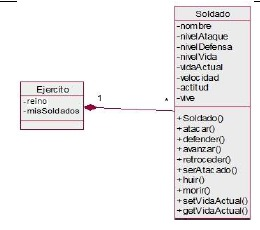
\includegraphics[height=10cm]{imagen.jpeg}
        \\
      
        \item la clase Main.java
        
        \begin{lstlisting}[language=java]
// RONI COMPANOCCA CHECCO
// CUI: 20210558
// LABORATORIO 12
import java.util.ArrayList;
import java.util.Collections;
import java.util.Comparator;

public class Main {

    public static void main(String[] args) {

		//DECLARACION DE VARIABLES Y ARREGLOS NECESARIOS
		ArrayList<Soldado> ejercito1 = new ArrayList();
		ArrayList<Soldado> ejercito2 = new ArrayList();
		ArrayList<ArrayList<Soldado>> tablero = new ArrayList();
		int batallon1, batallon2;
		int vidatotal1=0, vidatotal2=0;
		double promedioVida1=0, promedioVida2=0;

		// BUCLE PARA DESIGNAR LA CANTIDAD DE FILAS Y COLUMNAS DEL TABLERO
		for(int i=0; i<10; i++) {
			tablero.add(new ArrayList<Soldado>());
			for(int j=0; j<10; j++) {
				tablero.get(i).add(new Soldado());
			}
		}

		// CREACION DEL NUMERO DE POSICIONES DE CADA EJERCITO
		batallon1 = aleatorio(1,10);
		batallon2 = aleatorio(1,10);

		// INICIALIZAR ARREGLOS
		inicializarArreglo(ejercito1, batallon1);
		inicializarArreglo(ejercito2, batallon2);

		// GENERAR EJERCITOS VALIDOS
		generarEjercitos(ejercito1, ejercito2);

		// AÑADIR LOS EJERCITOS AL TABLERO
		añadirTablero(ejercito1, tablero);
		añadirTablero(ejercito2, tablero);

		//IMPRIMIR EL TABLERO
		imprimirTablero(tablero);

		//IMPRIMIR LOS SOLDADOS DE MAYOR VIDA DE CADA EJERCITO
		System.out.println("Soldado de mayor vida del ejercito 1");
		SoldadoConMayorVida(ejercito1);
		System.out.println("soldado de mayor vida del ejercito 2");
		SoldadoConMayorVida(ejercito2);

		//IMPRIMIR LA VIDA TOTAL Y EL PROMEDIO DEL EJERCITO 1
		System.out.println("\nEJERCITO 1: ");
		for (int i=0; i<ejercito1.size(); i++) {
			vidatotal1+=ejercito1.get(i).getPuntos();
			promedioVida1 = vidatotal1/(ejercito1.size()*1.0);
		}
		System.out.println("Vida total: "+vidatotal1);
		System.out.println("Promedio de vida: "+promedioVida1);
		
		//IMPRIMIR LA VIDA TOTAL Y EL PROMEDIO DEL EJERCITO 2
		System.out.println("\nEJERCITO 2: ");
		for (int i=0; i<ejercito2.size(); i++) {
			vidatotal2+=ejercito2.get(i).getPuntos();
			promedioVida2 = vidatotal2/(ejercito2.size()*1.0);
		}
		System.out.println("Vida total: "+vidatotal2);
		System.out.println("Promedio de vida: "+promedioVida2);

		//IMPRIMIR LOS SOLDADOS CREADOS EN EL ORDEN POR DEFECTO
		System.out.println("\nLista ejercito 1:");
		for(int i=0; i<ejercito1.size(); i++) {
			imprimir(ejercito1.get(i));
		}
		System.out.println("\nLista ejercito 2:");
		for(int i=0; i<ejercito2.size(); i++) {
			imprimir(ejercito2.get(i));
		}

		// IMPRIMIR LOS DATOS DE LOS SOLDADOS ORDENADOS DE MAYOR A MENOR DEPENDIENDO DE SU NIVEL DE VIDA USANDO DOS TIPOS DE ALGORITMO
		ordenarPorVidaMetodoA(ejercito1);
		ordenarPorVidaMetodoB(ejercito2);
		System.out.println("\nEjercito 1 Ordenados por nivel de vida");
		for(int i=0; i<ejercito1.size(); i++) {
			imprimir(ejercito1.get(i));
		}
		System.out.println("\nEjercito 2 Ordenados por nivel de vida");
		for(int i=0; i<ejercito2.size(); i++) {
			imprimir(ejercito2.get(i));
		}
		
		// MOSTRAR EJERCITO GANADOR LA METRICA USADA ARA DESIGNAR AL GANADOR ES POR EL NIVEL DEL PROMEDIO DE VIDA DE CADA EJERCITO
		if(promedioVida1>promedioVida2) {
			System.out.println("\nGANADOR ***EJERCITO 1***");
		}else if (promedioVida1<promedioVida2) {
			System.out.println("\nGANADOR ***EJERCITO 2***");
			}
		else {
			System.out.print("\n***ES UN EMPATE***");
		}
	}

    // METODO PARA CREAR NUMEROS ALEATORIOS EN UN RANGO
    public static int aleatorio(int min, int max) {
        return (int) (Math.random() * (max - min + 1) + min);
    }

    // METODO PARA INICIAR UN ARRAYLIST
    public static void inicializarArreglo(ArrayList<Soldado> soldadito, int num) {
        for (int i = 0; i < num; i++) {
            soldadito.add(new Soldado());
        }
    }

    // METODO PARA GENERAR DATOS DEL OBJETO SOLDADO
    public static Soldado generarDatos() {
        Soldado soldadito = new Soldado();
        soldadito.setNivelVida(aleatorio(1, 5));
        soldadito.setFila(aleatorio(1, 10));
        soldadito.setColumna(aleatorio(1, 10));
        return soldadito;
    }

    // METODOS PARA GENERAR LOS EJERCITOS DE MANERA ALEATORIA
    public static void generarEjercitos(ArrayList<Soldado> B1, ArrayList<Soldado> B2) {
        ArrayList<Soldado> Soldados = new ArrayList<>();
        Soldados.add(generarDatos());
        for (int i = 1; i < (B1.size() + B2.size()); i++) {
            Soldados.add(generarDatos());
            for (int j = 0; j < i; j++) {
                if (Soldados.get(i).getFila() == Soldados.get(j).getFila()) {
                    if (Soldados.get(i).getColumna() == Soldados.get(j).getColumna()) {
                        Soldados.remove(i);
                        i--;
                    }
                }
            }
        }
        for (int i = 0; i < B1.size(); i++) {
            B1.add(i, Soldados.get(i));
            B1.get(i).setNombre("Soldado" + i + "x1");
            B1.get(i).setActitud(B1.get(i).getNivelVida() + "[E1]");
            B1.remove(i + 1);
        }
        for (int i = 0; i < B2.size(); i++) {
            B2.add(i, Soldados.get(i + B1.size()));
            B2.get(i).setNombre("Soldado" + i + "x2");
            B2.remove(i + 1);
            B2.get(i).setActitud(B2.get(i).getNivelVida() + "[E2]");
        }
    }

    // METODO PARA AÑADIR LOS EJERCITOS AL TABLERO
    public static void añadirTablero(ArrayList<Soldado> soldadito, ArrayList<ArrayList<Soldado>> table) {
        for (int i = 0; i < soldadito.size(); i++) {
            table.get(soldadito.get(i).getColumna() - 1).add(soldadito.get(i).getFila() - 1, soldadito.get(i));
            table.get(soldadito.get(i).getColumna() - 1).remove(soldadito.get(i).getFila());
        }
    }

    // METODO PARA IMPRIMIR EL TABLERO EN LA CUAL SE DESARROLLA EL JUEGO
    public static void imprimirTablero(ArrayList<ArrayList<Soldado>> table) {
        System.out.println("\tA\tB\tC\tD\tF\tG\tH\tI\tJ");
        for (int i = 0; i < table.size(); i++) {
            System.out.print(i + 1);
            for (int j = 0; j < table.get(i).size(); j++) {
                System.out.print("\t" + table.get(i).get(j).getActitud());
            }
            System.out.println("\n");
        }
    }

    // METODO PARA IMPRIMIR LOS SOLDADOS DE MAYOR VIDA
    public static void SoldadoConMayorVida(ArrayList<Soldado> soldadito) {
        Soldado mayor = new Soldado();
        mayor.setNivelVida(0);
        for (int i = 0; i < soldadito.size(); i++) {
            if (mayor.getNivelVida() < soldadito.get(i).getNivelVida()) {
                mayor = soldadito.get(i);
            }
        }
        imprimir(mayor);
    }

    // METODO PARA IMPRIMIR EL NOMBRE, LA POSICION Y NIVEL DE VIDA DEL SOLDADO
    public static void imprimir(Soldado soldadito) {
        System.out.println("Nombre: " + soldadito.getNombre() + "\nPosicion: " + soldadito.getColumna() + "X" + soldadito.getFila() + "\tVida: " + soldadito.getNivelVida());
    }

    // METODO QUE NOS AYUDA A ORDENAR LOS SOLDADOS DE ACUERDO A SU NIVEL DE VIDA, USUANDO UN ALGORITMO DE ORDENAMIENTO DE BURBUJA
    public static void ordenarPorVidaMetodoA(ArrayList<Soldado> soldadito) {
        Soldado aux = new Soldado();
        for (int i = 0; i < soldadito.size() - 1; i++) {
            for (int j = 0; j < soldadito.size() - i - 1; j++) {
                if (soldadito.get(j).getNivelVida() < soldadito.get(j + 1).getNivelVida()) {
                    aux = soldadito.get(j);
                    soldadito.set(j, soldadito.get(j + 1));
                    soldadito.set(j + 1, aux);
                }
            }
        }
    }

    // METODO QUE NOS AYUDA A ORDENAR LOS SOLDADOS DE ACUERDO A SU NIVEL DE VIDA, EN ESTA OCACION DIFERENTE A LA ANTERIOR QUE ERA ALGORITMO DE BURBUJA
    public static void ordenarPorVidaMetodoB(ArrayList<Soldado> soldadito) {
        Collections.sort(soldadito, new Comparator<Soldado>() {
            public int compare(Soldado s1, Soldado s2) {
                // Orden descendente por nivel de vida
                return Integer.compare(s2.getNivelVida(), s1.getNivelVida());
            }
        });
    }
}
    // METODO PARA IMPRIMIR EL TABLERO EN LA CUAL SE DESARROLLA EL JUEGO
    public static void imprimirTablero(ArrayList<ArrayList<Soldado>> table) {
        System.out.println("\tA\tB\tC\tD\tF\tG\tH\tI\tJ");
        for (int i = 0; i < table.size(); i++) {
            System.out.print(i + 1);
            for (int j = 0; j < table.get(i).size(); j++) {
                System.out.print("\t" + table.get(i).get(j).getActitud());
            }
            System.out.println("\n");
        }
    }

    // METODO PARA IMPRIMIR LOS SOLDADOS DE MAYOR VIDA
    public static void SoldadoConMayorVida(ArrayList<Soldado> soldadito) {
        Soldado mayor = new Soldado();
        mayor.setNivelVida(0);
        for (int i = 0; i < soldadito.size(); i++) {
            if (mayor.getNivelVida() < soldadito.get(i).getNivelVida()) {
                mayor = soldadito.get(i);
            }
        }
        imprimir(mayor);
    }

    // METODO PARA IMPRIMIR EL NOMBRE, LA POSICION Y NIVEL DE VIDA DEL SOLDADO
    public static void imprimir(Soldado soldadito) {
        System.out.println("Nombre: " + soldadito.getNombre() + "\nPosicion: " + soldadito.getColumna() + "X" + soldadito.getFila() + "\tVida: " + soldadito.getNivelVida());
    }

    // METODO QUE NOS AYUDA A ORDENAR LOS SOLDADOS DE ACUERDO A SU NIVEL DE VIDA, USUANDO UN ALGORITMO DE ORDENAMIENTO DE BURBUJA
    public static void ordenarPorVidaMetodoA(ArrayList<Soldado> soldadito) {
        Soldado aux = new Soldado();
        for (int i = 0; i < soldadito.size() - 1; i++) {
            for (int j = 0; j < soldadito.size() - i - 1; j++) {
                if (soldadito.get(j).getNivelVida() < soldadito.get(j + 1).getNivelVida()) {
                    aux = soldadito.get(j);
                    soldadito.set(j, soldadito.get(j + 1));
                    soldadito.set(j + 1, aux);
                }
            }
        }
    }

    // METODO QUE NOS AYUDA A ORDENAR LOS SOLDADOS DE ACUERDO A SU NIVEL DE VIDA, EN ESTA OCACION DIFERENTE A LA ANTERIOR QUE ERA ALGORITMO DE BURBUJA
    public static void ordenarPorVidaMetodoB(ArrayList<Soldado> soldadito) {
        Collections.sort(soldadito, new Comparator<Soldado>() {
            public int compare(Soldado s1, Soldado s2) {
                // Orden descendente por nivel de vida
                return Integer.compare(s2.getNivelVida(), s1.getNivelVida());
            }
        });
    }
}
        \end{lstlisting}

        \item la clase Soldado.java
        \begin{lstlisting}[language=java]
// RONI COMPANOCCA CHECCO
// CUI: 20210558
// LABORATORIO 12
// FUNDAMENTOS DE PROGRAMACION 
// CLASE SOLDADO PARA LOS METODOS SETTER Y GETTER
public class Soldado {
    private String nombre;
    private int nivelAtaque;
    private int nivelDefensa;
    private int nivelVida;
    private int vidaActual;
    private int velocidad;
    private String actitud;
    private boolean vive;

    public Soldado() {
        nombre = "";
        nivelAtaque = 0;
        nivelDefensa = 0;
        nivelVida = 0;
        vidaActual = nivelVida;
        velocidad = 0;
        actitud = "";
        vive = true;
    }

    public void atacar(Soldado enemigo) {
        int danio = this.nivelAtaque - enemigo.nivelDefensa;
        if (danio > 0) {
            enemigo.serAtacado(danio);
            System.out.println(this.nombre + " atacó a " + enemigo.nombre + " y le causó " + danio + " de daño.");
        } else {
            System.out.println(this.nombre + " atacó a " + enemigo.nombre + " pero no le causó daño.");
        }
    }

    public void defender() {
        // Lógica para la defensa
        // Puede disminuir el daño recibido en un futuro ataque, por ejemplo
        this.nivelDefensa += 10; // Aumentar la defensa por ejemplo
        System.out.println(this.nombre + " se está defendiendo.");
    }

    public void avanzar() {
        // Lógica para avanzar en el juego
        // Podría mover al soldado a una nueva posición en el tablero, por ejemplo
        if (this.velocidad > 0) {
            // Mover al soldado en la dirección correspondiente
            System.out.println(this.nombre + " está avanzando.");
        } else {
            System.out.println(this.nombre + " no puede avanzar, la velocidad es 0.");
        }
    }

    public void retroceder() {
        // Lógica para retroceder en el juego
        // Podría mover al soldado hacia atrás en el tablero, por ejemplo
        System.out.println(this.nombre + " está retrocediendo.");
    }

    public void serAtacado(int danioRecibido) {
        this.vidaActual -= danioRecibido;
        if (this.vidaActual <= 0) {
            this.morir();
        }
    }

    public void huir() {
        // Lógica para huir del combate
        // Podría cambiar la posición del soldado a una zona segura, por ejemplo
        if (this.nivelVida < 10) {
            // Huir solo si la vida es baja
            System.out.println(this.nombre + " está huyendo del combate.");
        } else {
            System.out.println(this.nombre + " no puede huir, su vida está alta.");
        }
    }

    public void morir() {
        this.vidaActual = 0;
        this.vive = false;
    }

    public void setVidaActual(int vidaActual) {
        this.vidaActual = vidaActual;
    }

    public int getVidaActual() {
        return vidaActual;
    }

    // Getters y Setters

    public String getNombre() {
        return nombre;
    }

    public String getNivelVida() {
        return nivelVida;
    }

    public void setNombre(String nombre) {
        this.nombre = nombre;
    }

    public int getNivelAtaque() {
        return nivelAtaque;
    }

    public int setNivelVida() {
        this.nivelVida = nivelVida;
    }

    public void setNivelAtaque(int nivelAtaque) {
        this.nivelAtaque = nivelAtaque;
    }

    public int getNivelDefensa() {
        return nivelDefensa;
    }

    public void setNivelDefensa(int nivelDefensa) {
        this.nivelDefensa = nivelDefensa;
    }

    public boolean isVive() {
        return vive;
    }

    public void setVive(boolean vive) {
        this.vive = vive;
    }
}
        \end{lstlisting}

        
        \item Ejecucion
        \begin{lstlisting}[language=java]
            A       B       C       D       F       G       H       I       J
1                                               2[E1]

2                                                               5[E1]

3

4

5

6                                                                       2[E2]

7

8                               2[E1]   3[E2]

9       3[E2]                                                           2[E1]

10                                              2[E1]           3[E2]

Soldado de mayor vida del ejercito 1
Nombre: Soldado4x1
Posicion: 2X8   Vida: 5
soldado de mayor vida del ejercito 2
Nombre: Soldado0x2
Posicion: 10X8  Vida: 3

EJERCITO 1:
Vida total: 13
Promedio de vida: 2.6

EJERCITO 2:
Vida total: 11
Promedio de vida: 2.75

Lista ejercito 1:
Nombre: Soldado0x1
Posicion: 1X6   Vida: 2
Nombre: Soldado1x1
Posicion: 9X9   Vida: 2
Nombre: Soldado2x1
Posicion: 8X4   Vida: 2
Nombre: Soldado3x1
Posicion: 10X6  Vida: 2
Nombre: Soldado4x1
Posicion: 2X8   Vida: 5

Lista ejercito 2:
Nombre: Soldado0x2
Posicion: 10X8  Vida: 3
Nombre: Soldado1x2
Posicion: 8X5   Vida: 3
Nombre: Soldado2x2
Posicion: 6X9   Vida: 2
Nombre: Soldado3x2
Posicion: 9X1   Vida: 3

Ejercito 1 Ordenados por nivel de vida
Nombre: Soldado4x1
Posicion: 2X8   Vida: 5
Nombre: Soldado0x1
Posicion: 1X6   Vida: 2
Nombre: Soldado1x1
Posicion: 9X9   Vida: 2
Nombre: Soldado2x1
Posicion: 8X4   Vida: 2
Nombre: Soldado3x1
Posicion: 10X6  Vida: 2

Ejercito 2 Ordenados por nivel de vida
Nombre: Soldado0x2
Posicion: 10X8  Vida: 3
Nombre: Soldado1x2
Posicion: 8X5   Vida: 3
Nombre: Soldado3x2
Posicion: 9X1   Vida: 3
Nombre: Soldado2x2
Posicion: 6X9   Vida: 2

GANADOR ***EJERCITO 2***
        \end{lstlisting}

    
	\end{itemize}
	\begin{itemize}
        \textcolor{red}{PROBLEMA 02}
        \\
        \\
        \item Basándose en los laboratorios anteriores
        \\
        \\
        \item Crear la clase Mapa, que esté constituida por el tablero antes visto, pero que en lugar de soldados, posicione ejércitos en ciertas posiciones aleatorias (entre 1 y 10 ejércitos por cada reino). Se deben generar ejércitos de 2 reinos, entre 1 y 10 soldados por ejército. No se admite guerra civil. El Mapa tiene como atributo el tipo de territorio que puede ser (bosque, campo abierto, montaña, desierto, playa). La cantidad de ejércitos y cantidad de soldados por ejército, así como todos sus atributos se deben generar aleatoriamente
        \\
        \\
        \item Dibujar el Mapa con las restricciones que sólo 1 ejercito como máximo en cada cuadrado
        \\
        \\
        \item El mapa tiene un solo tipo de territorio autogenerado
        \\
        \\
        \item Considerar que el territorio influye en los resultados de las batallas, así cada reino tiene bonus según el territorio: Inglaterra->bosque, Francia->campo abierto, Castilla-Aragón->montaña, Moros->desierto, Sacro Imperio RomanoGermánico->bosque, playa y campo abierto. En dichos casos, se aumenta el nivel de vida en 1 a todos los soldados del reino beneficiado
        \\
        \\
        \item Realizar el diagrama de clases de UML completo
        \\
        \\
        \item Indicar quién ganaría la guerra y justificar por qué. Describir 3 métricas usadas
        \\
        \\
        \item Hacerlo iterativo
        \\
        \\
        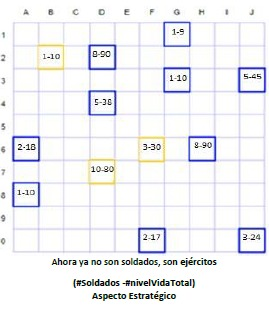
\includegraphics[height=10cm]{imagen1.jpeg}

	\end{itemize}

    \section{REFERENCIAS}
	\begin{itemize}
		\item ¿Qué son la propiedades y métodos de instancia, qué diferencia tienen con las propiedades y métodos de clase?
        \\
        \text En la programación orientada a objetos, tanto en lenguajes como Python, Java, C++, entre otros, se utilizan conceptos como propiedades y métodos de instancia, así como propiedades y métodos de clase. Estos conceptos son fundamentales para entender la estructura y el comportamiento de las clases.
		\item ¿Qué ventajas tiene la relación de herencia?
        \\
        \text La herencia es uno de los conceptos fundamentales de la programación orientada a objetos (POO) y proporciona varias ventajas en el diseño y desarrollo de software. 
		\item ¿Qué es la sobreescritura y la sobrecarga de métodos?
        \\
        \text La sobreescritura de métodos ocurre cuando una clase hija proporciona una implementación específica para un método que ya está definido en su clase base (o en una de sus clases ancestrales). La firma del método (nombre y parámetros) en la clase hija es la misma que la firma en la clase base. La sobreescritura permite a las clases hijas proporcionar su propia implementación del método, reemplazando así la implementación de la clase base.
	\end{itemize}
	\section{REFERENCIAS}
	\begin{itemize}
		\item M. Aedo, “Fundamentos de Programación 2 - Tópicos de Programación Orientada a Objetos”, Primera Edición, 2021, Editorial UNSA.
		\item \url{https://github.com/rescobedoq/programacion.git}
		\item J. Dean, "Introduction to programming with Java: A Problem Solving Approach”, Third Edition, 2021, McGraw-Hill.
        \item C. T. Wu, "An Introduction to Object-Oriented Programming with Java", Fifth Edition, 2010, McGraw-Hill.
        \item P. Deitel, "Java How to Program", Eleventh Edition, 2017, Prentice Hall.
	\end{itemize}
	
%\clearpage
%\bibliographystyle{apalike}
%\bibliographystyle{IEEEtranN}
%\bibliography{bibliography}
			
\end{document}